\chapter{Measurement of the \texorpdfstring{\ce{^{64}Zn}, \ce{^{47}Ti}}{64Zn, 47Ti}(n,p) cross sections using a DD neutron generator for medical isotope studies}\label{sec:chapter_hfng}
% \Capinsertold This chapter 
\chaptermark{Measurement of the \texorpdfstring{\ce{^{64}Zn}, \ce{^{47}Ti}}{64Zn, 47Ti}(n,p) cross sections}


\Capinsert[4]{\textbf{T}}{his} chapter details a measurement of the \ce{^{64}Zn}(n,p)\ce{^{64}Cu} and \ce{^{47}Ti}(n,p)\ce{^{47}Sc} cross sections.
The measurement was performed using the UC Berkeley High Flux Neutron Generator (HFNG), a compact generator which produces a neutron flux through the DD fusion reaction.
This generator, commissioned in 2015, was originally designed for radiometric dating applications in geochronology, with an emphasis on the \ce{^{40}Ar}/\ce{^{39}Ar} dating technique.
While other experiments have been carried out at the HFNG since this work was published, the work presented in this chapter was the first scientific measurement to be carried out in this new research facility.
In addition to the pivotal role played in the early development of the HFNG, this work is notable for several aspects related to the development of alternative production pathways for medical radionuclides.

For isotopes accessible through (n,p) production channels, the use of neutrons in the 2--3\,MeV DD spectrum provides a nearly ideal pathway for high specific activity production.
This is due to the fact that the DD neutron spectrum is too slow for production of unwanted activities via (n,pxn) and (n,$\alpha$xn) reactions, which cannot easily be separated from the desired radionuclides. 
DT generators offer higher production rates through increased  neutron flux, but their more-energetic neutron spectra suffer from the opening of production channels for many unwanted radionuclide contaminants.
In addition, especially in a generator with a low thermal neutron population such as the HFNG, the DD spectrum is too energetic for  neutron capture to be competitive with (n,p) reaction rates.
Production of multiple unwanted co-activities via (n,$\gamma$) is one of the largest issues faced by thermal reactor isotope production.
This is primarily due to the separation of a single radionuclide product from this \enquote{sea} of contaminant co-products being impractical by radiochemical means, and often impossible by affordable means.
As a result, reactor production suffers from low radioisotopic purity, as well as yields of low specific activity.
In addition, production reactors suffer from difficulties with large-scale deployment due to their reliance on highly-enriched uranium, and  a global trend currently exists for the curtailment of such reactors.


These factors combine to make alternative pathways to reactor production a highly-sought goal for the field of nuclear medicine.
The potential for high-specific activity production and easy deployment, due to compact size and lack of dependence on special nuclear material, allows a DD neutron generator to stand poised as a novel paradigm for isotope production.
A challenge to wider utilization of  such generators  is the paucity of well-characterized nuclear data for the production of isotopes via (n,p) and (n,$\alpha$) channels.
This motivated the work described here, as a feasibility study for the use of compact DD neutron generators for nuclear data measurements, as well as the potential for serving as local medical isotope production capabilities.
The design, commissioning, and operation of the HFNG has been the product of the time and efforts of numerous individuals, including three generations of PhD students at the UC Berkeley Department of Nuclear Engineering. 
These efforts culminated in the work presented in this chapter, the result of the first characterization experiments  at the HFNG.
Part of this characterization includes the description of a new figure of merit for isotope production in a neutron generator, $\eta$, the \emph{neutron utilization factor,}.
This figure  characterizes the effectiveness of a neutron generator for the production of a specific isotope, based on target configuration and reaction selectivity.


\vspace{1cm}



\noindent \textbf{Relevant Publications:}

\vspace{0.5cm}


\hangindent=\parindent  \textbf{A.S. Voyles}, M.S. Basunia, J.C. Batchelder, J.D. Bauer, T.A. Becker, L.A. Bernstein, E.F. Matthews, P.R. Renne, D. Rutte, M.A. Unzueta, and K.A. van Bibber, \enquote{Measurement of the \ce{^{64}Zn}, \ce{^{47}Ti}(n,p) cross sections using a DD neutron generator for medical isotope studies,} Nuclear Instruments and Methods in Physics Research Section B: Beam Interactions with Materials and Atoms, vol. 410, pp. 230--239, Nov. 2017, \url{http://dx.doi.org/10.1016/j.nimb.2017.08.021}. \cite{Voyles2017} 

% T.H. Joshi, S. Sangiorgio, V. Mozin, E.B. Norman, P. Sorensen, M. Foxe, G. Bench, A. Bernstein. Design and characterization of a quasi-monoenergetic neutron source. Nuclear Instruments and Methods in Physics Research B (in press). [44]

\vspace{0.5cm}



The text and figures of this paper (copyright Elsevier B.V. 2017), of which I was the primary author, are
included in this chapter with the permission of all authors. 
Some of the figures and and content in this chapter have been altered to better fit the page formatting, but all changes made to the published journal article are purely stylistic in nature.


% \lstinputlisting[basicstyle=\small,linewidth=\columnwidth,
% % language=Python,
% language=MCNP6,
% breaklines=true,frame=single]{./codes/HFNGSimp9PDCR39.txt}



% % 
% 
%  Dump body text from HFNG (n,p) paper into this chapter
% 
% % 
\section{Abstract}
\input{../Manuscripts/First_np_Paper/np_abstract_text}


% % 
% 
%  Dump body text from HFNG (n,p) paper into this chapter
% 
% % 
\input{../Manuscripts/First_np_Paper/np_body_text}



%
% Additional figures
% 
\section{Additional discussion} \label{sec:extra_np}

Additional discussion of the experimental and analytical details for this work, which were excluded from the published journal article to preserve its scope, are included here.



The basic design characteristics and operation of the HFNG have been described in this chapter, but a more detailed discussion of the generator may be found in the recent work of Ayllon \etal\ \cite{ayllon2018design}. 
% \textred{Update this BibTeX reference following acceptance!}
The HFNG is seen in  \autoref{fig:alt_HFNG}, illustrating the compact nature of the generator.
A photograph of the actual sample holder used for the HFNG irradiations in this chapter is seen in \autoref{fig:holder_c}, for the case of a  \ce{^{64}Zn}(n,p)\ce{^{64}Cu} measurement.


\begin{figure}
    \centering
%         \includegraphics[width=\columnwidth]{./figures/Capture.PNG}
        \includegraphics[height=2.75in,angle=90]{./figures/IMG_20151103_113432563.jpg}
        \caption{Sample holder used for the Berkeley HFNG. The zinc (visible) foil is co-loaded on top of reference indium foil, ready for irradiation.}
        \label{fig:holder_c}
\end{figure}


\begin{figure}
 \centering
%  \includegraphics[width=\columnwidth]{./figures/IMG_20160531_183154957_HDR.jpg}
%  \includegraphics[scale=0.06]{./figures/IMG_20160531_183154957_HDR.jpg}
 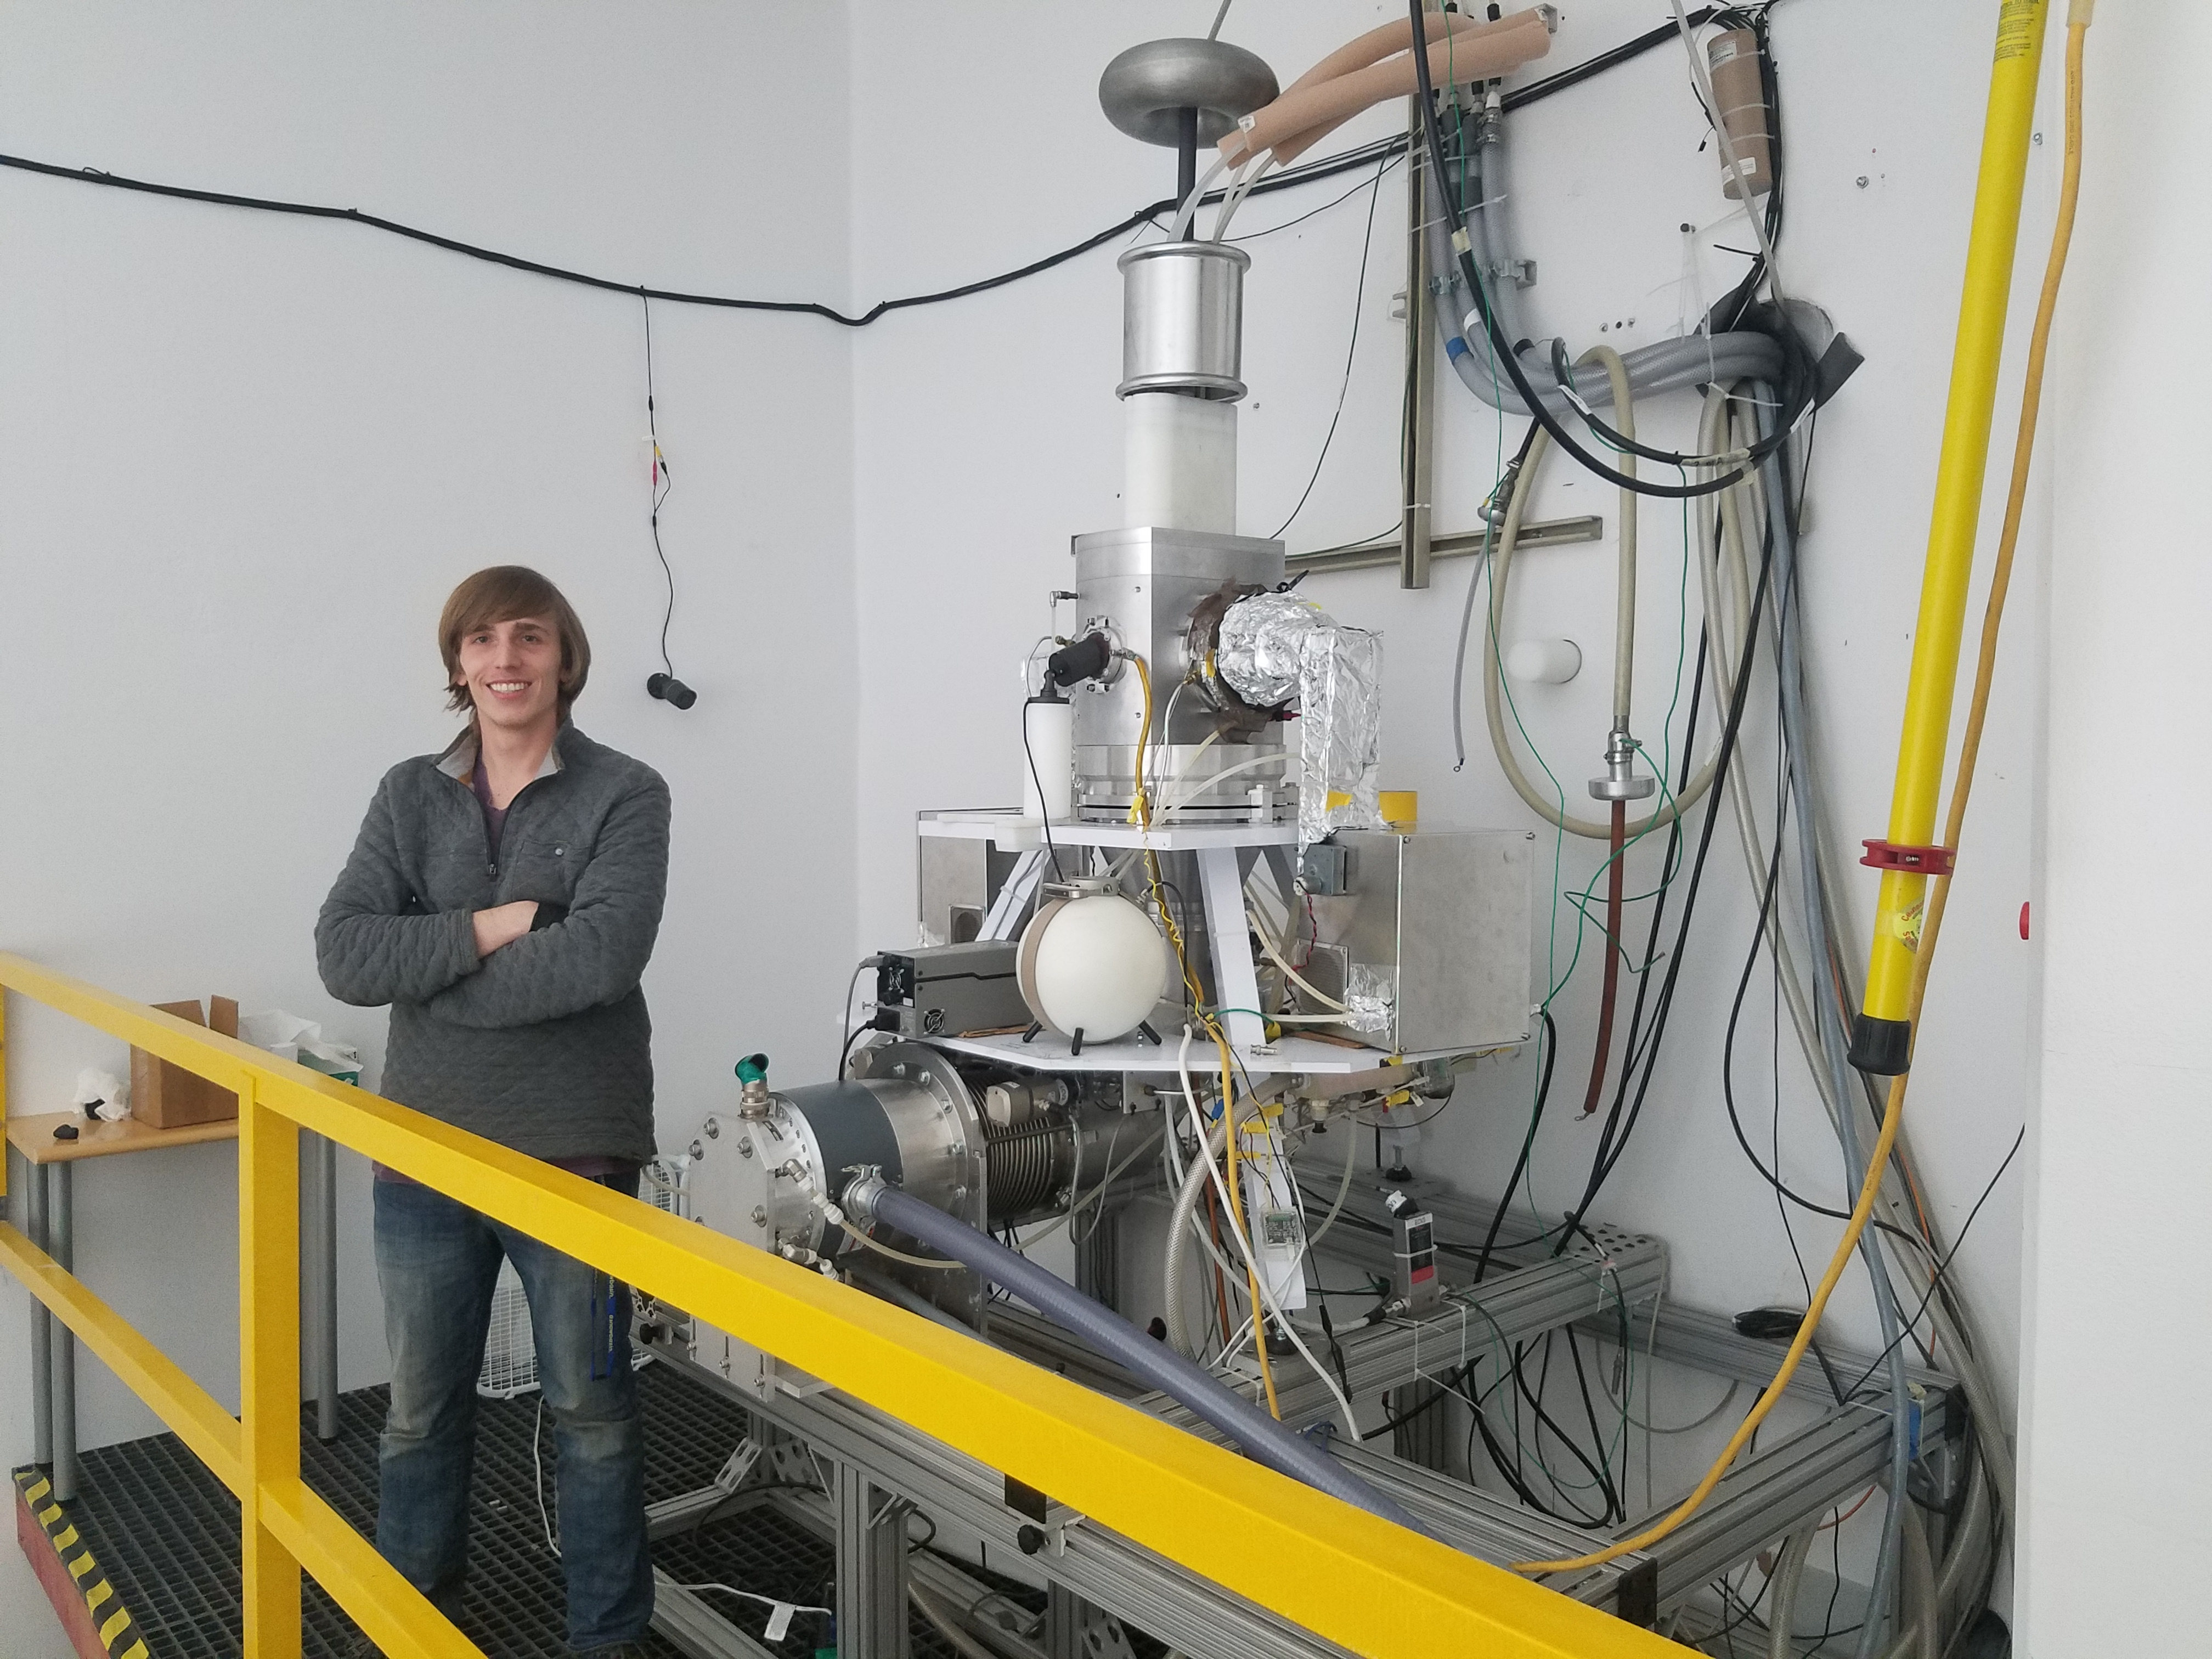
\includegraphics[width=0.75\columnwidth]{./figures/new_hfng_photo.jpg}
 % IMG_20160531_183154957_HDR.jpg: 2432x4320 pixel, 72dpi, 85.80x152.40 cm, bb=0 0 2432 4320
 \caption{The UC Berkeley High-Flux Neutron Generator, along with  UC Berkeley Nuclear Engineering PhD student Jon Morrell, who currently leads operation of the HFNG.}
 \label{fig:alt_HFNG}
\end{figure}


A rendering of the HFNG target chamber, as modeled in MCNP6, is seen in \autoref{fig:mcnp_vised}.
This figure presents a small subset of the full MCNP6 model of the HFNG,  to better illustrate the geometry of the target chamber.
This model is the same described in \autoref{sec:n_source} for simulation of neutron transport in the HFNG.
The full input file for this MCNP model is included here for reference, in Appendix \ref{sec:hfng_mcnp_deck}.









\begin{figure}
 \centering
 %trim option's parameter order: left bottom right top
 \includegraphics[trim = 0mm 10mm 2mm 10mm, clip,width=0.75\columnwidth]{./figures/mcnp_vised2.png}
 % mcnp_vised2.PNG.png: 688x443 pixel, 96dpi, 18.21x11.72 cm, bb=0 0 516 332
 \caption{MCNP6 model of the HFNG target chamber, with reference scale. The co-loaded foils can be seen in the target chamber center.  The ovals indicate the location of water cooling channels.}
 \label{fig:mcnp_vised}
\end{figure}






\begin{figure*}
    \centering
    \subfloat{
        \centering
%         \includegraphics[width=\columnwidth]{./figures/Capture.PNG}
%         \subfigimg[width=0.495\textwidth]{a)}{./figures/IMG_20160531_182618557_HDR.jpg}{50}
        \subfigimg[height=2.7in]{a)}{./figures/IMG_20160531_182618557_HDR.jpg}{20}
%         \caption{ Decay curve for the isomeric transition of \ce{^{115m}In}.}
%          \refstepcounter{subfloat}
         \label{fig:hpge_a}
%          
%          \subfigimg[width=0.495\textwidth]{b)}{./figures/IMG_20160531_182635712_HDR.jpg}{50}
         \subfigimg[height=2.7in]{b)}{./figures/IMG_20160531_182635712_HDR.jpg}{50}
%         \caption{ Decay curve for the isomeric transition of \ce{^{113m}In}.}
%          \refstepcounter{subfloat}
         \label{fig:hpge_b}
    }%
    \caption{High-Purity Germanium Detectors used for gamma spectroscopy of the activated foils, as described in \autoref{sec:spectroscopy_np}. (a) Ortec 80\% HPGe detector, (b) Ortec planar LEPS detector.}
     \label{fig:main_ge_detectors}
\end{figure*}



As described in \autoref{sec:spectroscopy_np}, the activities produced in the HFNG irradiations were quantified via gamma-ray spectrometry.
Two detectors were used in this measurement.
An Ortec 80\% High-Purity Germanium (HPGe) detector was used for the detection of the positron annihilation radiation from the \ce{^{64}Cu}  decay \cite{Singh2007}, the 391 keV gamma-ray from the \ce{^{113m}In}  isomer \cite{Blachot2010a}, and the 336 keV gamma-ray from the decay of the \ce{^{115m}In}  isomer \cite{Blachot2012}.
An Ortec planar Low-Energy Photon Spectrometer (LEPS)  was used for the detection of the lower-energy 159 keV gamma-ray from \ce{^{47}Sc} \cite{Burrows2007} as well as the two indium isomers mentioned above.
Both of these detectors are seen in \autoref{fig:main_ge_detectors}.




It is worth mentioning that, since natural zinc has five stable isotopes (\ce{^{64,66-68,70}Zn} \cite{Meija2016}), one would expect to see  
% (n,p) 
reaction channels on all five isotopes. 
% in the DD neutron spectrum.
Indeed, \ce{^{66}Zn}(n,p)\ce{^{66}Cu} has an energetic threshold of 1.886\,MeV, but was not seen in the work described here, due to the reaction having a very weak cross section at these energies  (approximately 0.2\,mb \cite{Smith1980}), and a short-lived product ($t_{1/2}=5.120\pm0.014$\,m \cite{Browne2010a}).
Operating protocol requires a 30 minute delay between shutdown and entrance to the HFNG vault, to allow for short-lived and airborne reaction products to decay out, and reduce prompt dose rates.
However, this makes quantification difficult for any reaction products with lifetimes less than approximately 15 minutes. 
\ce{^{68}Zn}(n,p)\ce{^{68}Cu} ($t_{1/2}=30.9\pm0.6$\,s \cite{McCutchan2012}) is not observed due to the DD spectrum being below the energetic threshold of 3.712\,MeV.
A similar argument holds for \ce{^{70}Zn}(n,p)\ce{^{70}Cu} ($t_{1/2}=44.5\pm0.2$\,s \cite{Gurdal2016}, threshold 5.889\,MeV) --- though both of these products would have decayed back into Zn long before the samples were removed from the HFNG.


However, none of these arguments apply to the case of \ce{^{67}Zn}(n,p)\ce{^{67}Cu} ($t_{1/2}=61.83\pm0.12$\,h \cite{Junde2005}), which is not short-lived, and has a positive reaction Q-value of 221.55\,keV.
Weak  \ce{^{67}Cu} activities were indeed seen in the gamma spectrometry of the activated zinc targets, but no \ce{^{67}Zn}(n,p)\ce{^{67}Cu} cross sections were reported.
% This is because 
\ce{^{67}Cu} activity could not be quantified with sufficient confidence for the reporting of a cross section, especially one with significant medical applications. 
This is due to the low natural abundance (4.04\%)  of \ce{^{67}Zn}, combined with its weak cross section of approximately 1.5\,mb at this energy \cite{Shimizu2004975}.
In addition, at the time of the published work, HFNG operation was limited to irradiations with maximum durations of approximately three hours.
\ce{^{67}Cu} is highly desired as part of a theranostic pair with \ce{^{64}Cu}, but no satisfactory production routes currently are available.
Indeed, \ce{^{67}Zn}(n,p)\ce{^{67}Cu} via fission neutrons has discrepant production data and extremely low radiochemical purity, and \ce{^{68}Zn}($\gamma$,p)\ce{^{67}Cu}, \ce{^{70}Zn}(p,$\alpha$)\ce{^{67}Cu}, and \ce{^{68}Zn}(p,2p)\ce{^{67}Cu} all suffer from low yields, and require enriched targets for radioisotopic purity \cite{Qaim201731}.
% and nuclear data for \ce{^{67}Cu} production is sparse. 
\ce{^{67}Zn}(n,p)\ce{^{67}Cu} data are extremely sparse in the 1--5\, MeV region, with only 7 measured data points \cite{VanLoef1961,Shimizu2004975,Furuta2008,Bhike2009}.
It is clear that a repeated measurement of the \ce{^{67}Zn}(n,p)\ce{^{67}Cu} cross section at the HFNG would be a useful endeavor, especially irradiating a target enriched in \ce{^{67}Zn}.
With recent generator upgrades, it is capable of sustaining irradiations up to a few days in length --- such an irradiation would be able to drive a zinc target much closer to the \ce{^{67}Cu} saturation activity, permitting this valuable measurement.





A similar argument can be made for the other \ce{^{nat}Ti}(n,p) channels.
\ce{^{46}Ti}(n,p)\ce{^{46}Sc} is energetically permitted, but was not observed --- indeed, this cross section has not been observed below 3.6\,MeV \cite{Smith1975}.
Much like \ce{^{67}Cu}, this measurement could easily be re-attempted using a longer irradiation ($t_{1/2}=83.79\pm0.04$\,d \cite{Wu2000}) and an enriched target (8.25\%  natural \ce{^{46}Ti} abundance).
\ce{^{48}Ti}(n,p)\ce{^{48}Sc} and \ce{^{50}Ti}(n,p)\ce{^{50}Sc} are inaccessible, as the DD spectrum falls below their energetic threshold of 3.273\,MeV and 6.225\,MeV, respectively.
\ce{^{49}Ti}(n,p)\ce{^{49}Sc} would be difficult to measure due to a lack of strong decay gamma-rays, but could be quantified via its 824.1\,keV $\beta^-$ emission ($I_\beta=99.940\%$) using liquid scintillation spectrometry  \cite{Burrows2008}.


\subsubsection{Recent and future HFNG experiments}



The characterization described in this chapter has  served as the basis for more recent measurements at the HFNG.
The characterized energy spectrum and MCNP neutron transport model described here, along with experience gained in these measurements, have provided guidance for suitable experiments accessible at the HFNG facility.
Two such recent experiments are described here.




% New measurement of the 35 Cl(n,x) cross sections for Molten Salt Reactor Design
Many proposed designs for molten salt reactors use chlorine-based salts as coolant. 
Unfortunately, the \ce{^{35}Cl}(n,p) reaction is a significant neutron \enquote{poison}, consuming fast spectrum neutrons needed to achieve criticality and producing the long-lived \ce{^{35}S} ($t_{1/2}=87.37\pm0.04$\,d \cite{Chen2011}). 
In addition to the \ce{^{35}Cl}(n,p) reaction, \ce{^{35}Cl}(n,$\alpha$) produces \ce{^{32}P}  ($t_{1/2}=14.268\pm0.005$\,d \cite{Ouellet2011}) which is used as a radiochemical tracer for metabolic studies. 
Unfortunately, no measurements  of this important cross section exist between 100\,keV and 14.1\,MeV incident neutron energy.
To this end, we performed an activation experiment using reagent-grade NaCl together with a \ce{^{nat}In} monitor. 
Preliminary results from this experiment have indicated a value far lower than in evaluated libraries, prompting a
second series of measurements at a range of angles to determine the energy dependence of the cross section near 2.7\,MeV. This result will not only inform future \ce{^{35}Cl} cross section evaluations, but will also provide a probe of transition
between the Resolved and Unresolved Resonance energy regions and the energies where statistical models are expected to be more appropriate.



\ce{^{99m}Tc} is one of the most well-known medical radionuclides, used as a diagnostic isotope in cardiac, renal, lung function, and tumor imaging studies.
Collected in a \ce{^{99}Mo}/\ce{^{99m}Tc} generator system, the \ce{^{99}Mo} parent has traditionally been produced as a fission product in thermal reactors.
However, an aging reactor fleet and proliferation concerns associated with \ce{^{99}Mo} recovery have recently made the identification of alternative production pathways one of the highest priorities in the nuclear data community \cite{bernstein2015nuclear}.
DD neutron generators stand poised as one such possible alternative, through production via the \ce{^{98}Mo}(n,$\gamma$)\ce{^{99}Mo} reaction.
A recent measurement was performed at the HFNG to measure  the energy dependence of this cross section  at four energy locations near 2.7\,MeV.
The custom holder designed for this measurement  is seen in \autoref{fig:mo_4foils}.
This cross section has not been measured since 1967 \cite{Stupegia1968}  and re-measurement  in the 1--10 MeV region has been  listed as a vital nuclear data need  for  \ce{^{99}Mo}  production.


\begin{figure}
 \centering
%                                l   b      r    top
%  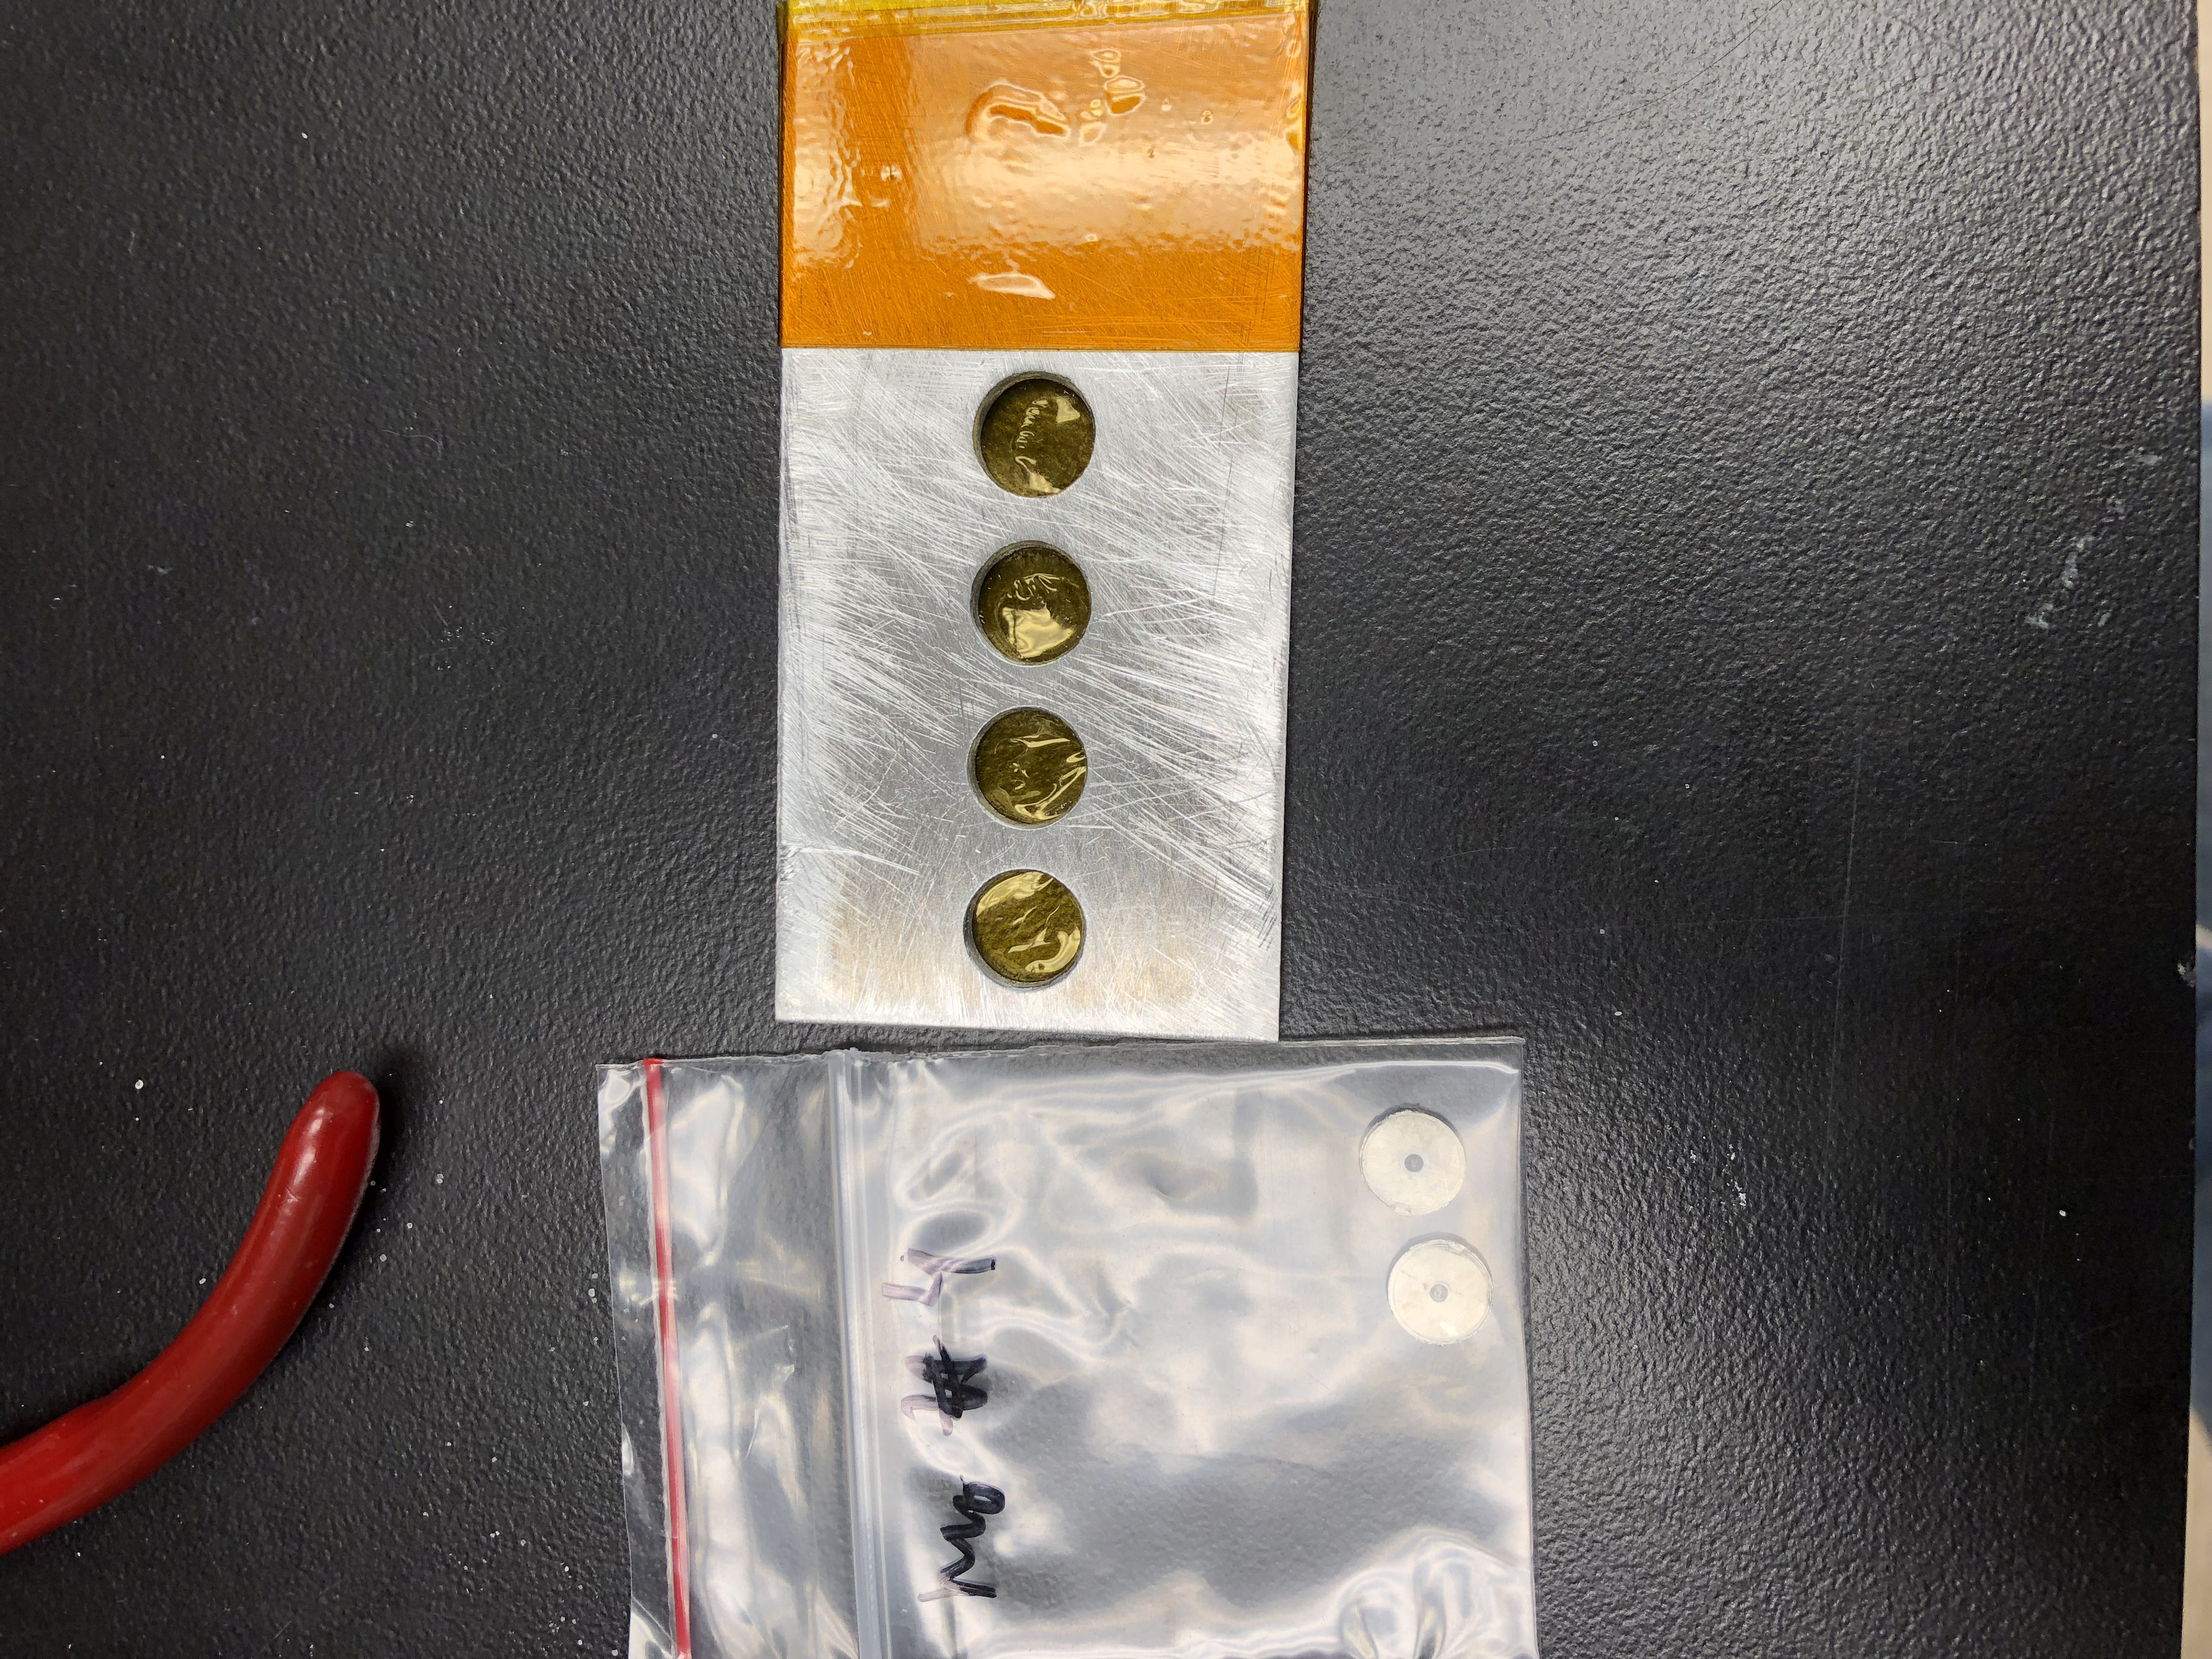
\includegraphics[clip=true,trim=5pt 1000pt 10pt 900pt,width=0.75\columnwidth,angle=90]{./figures/IMG_8840.JPG}
%  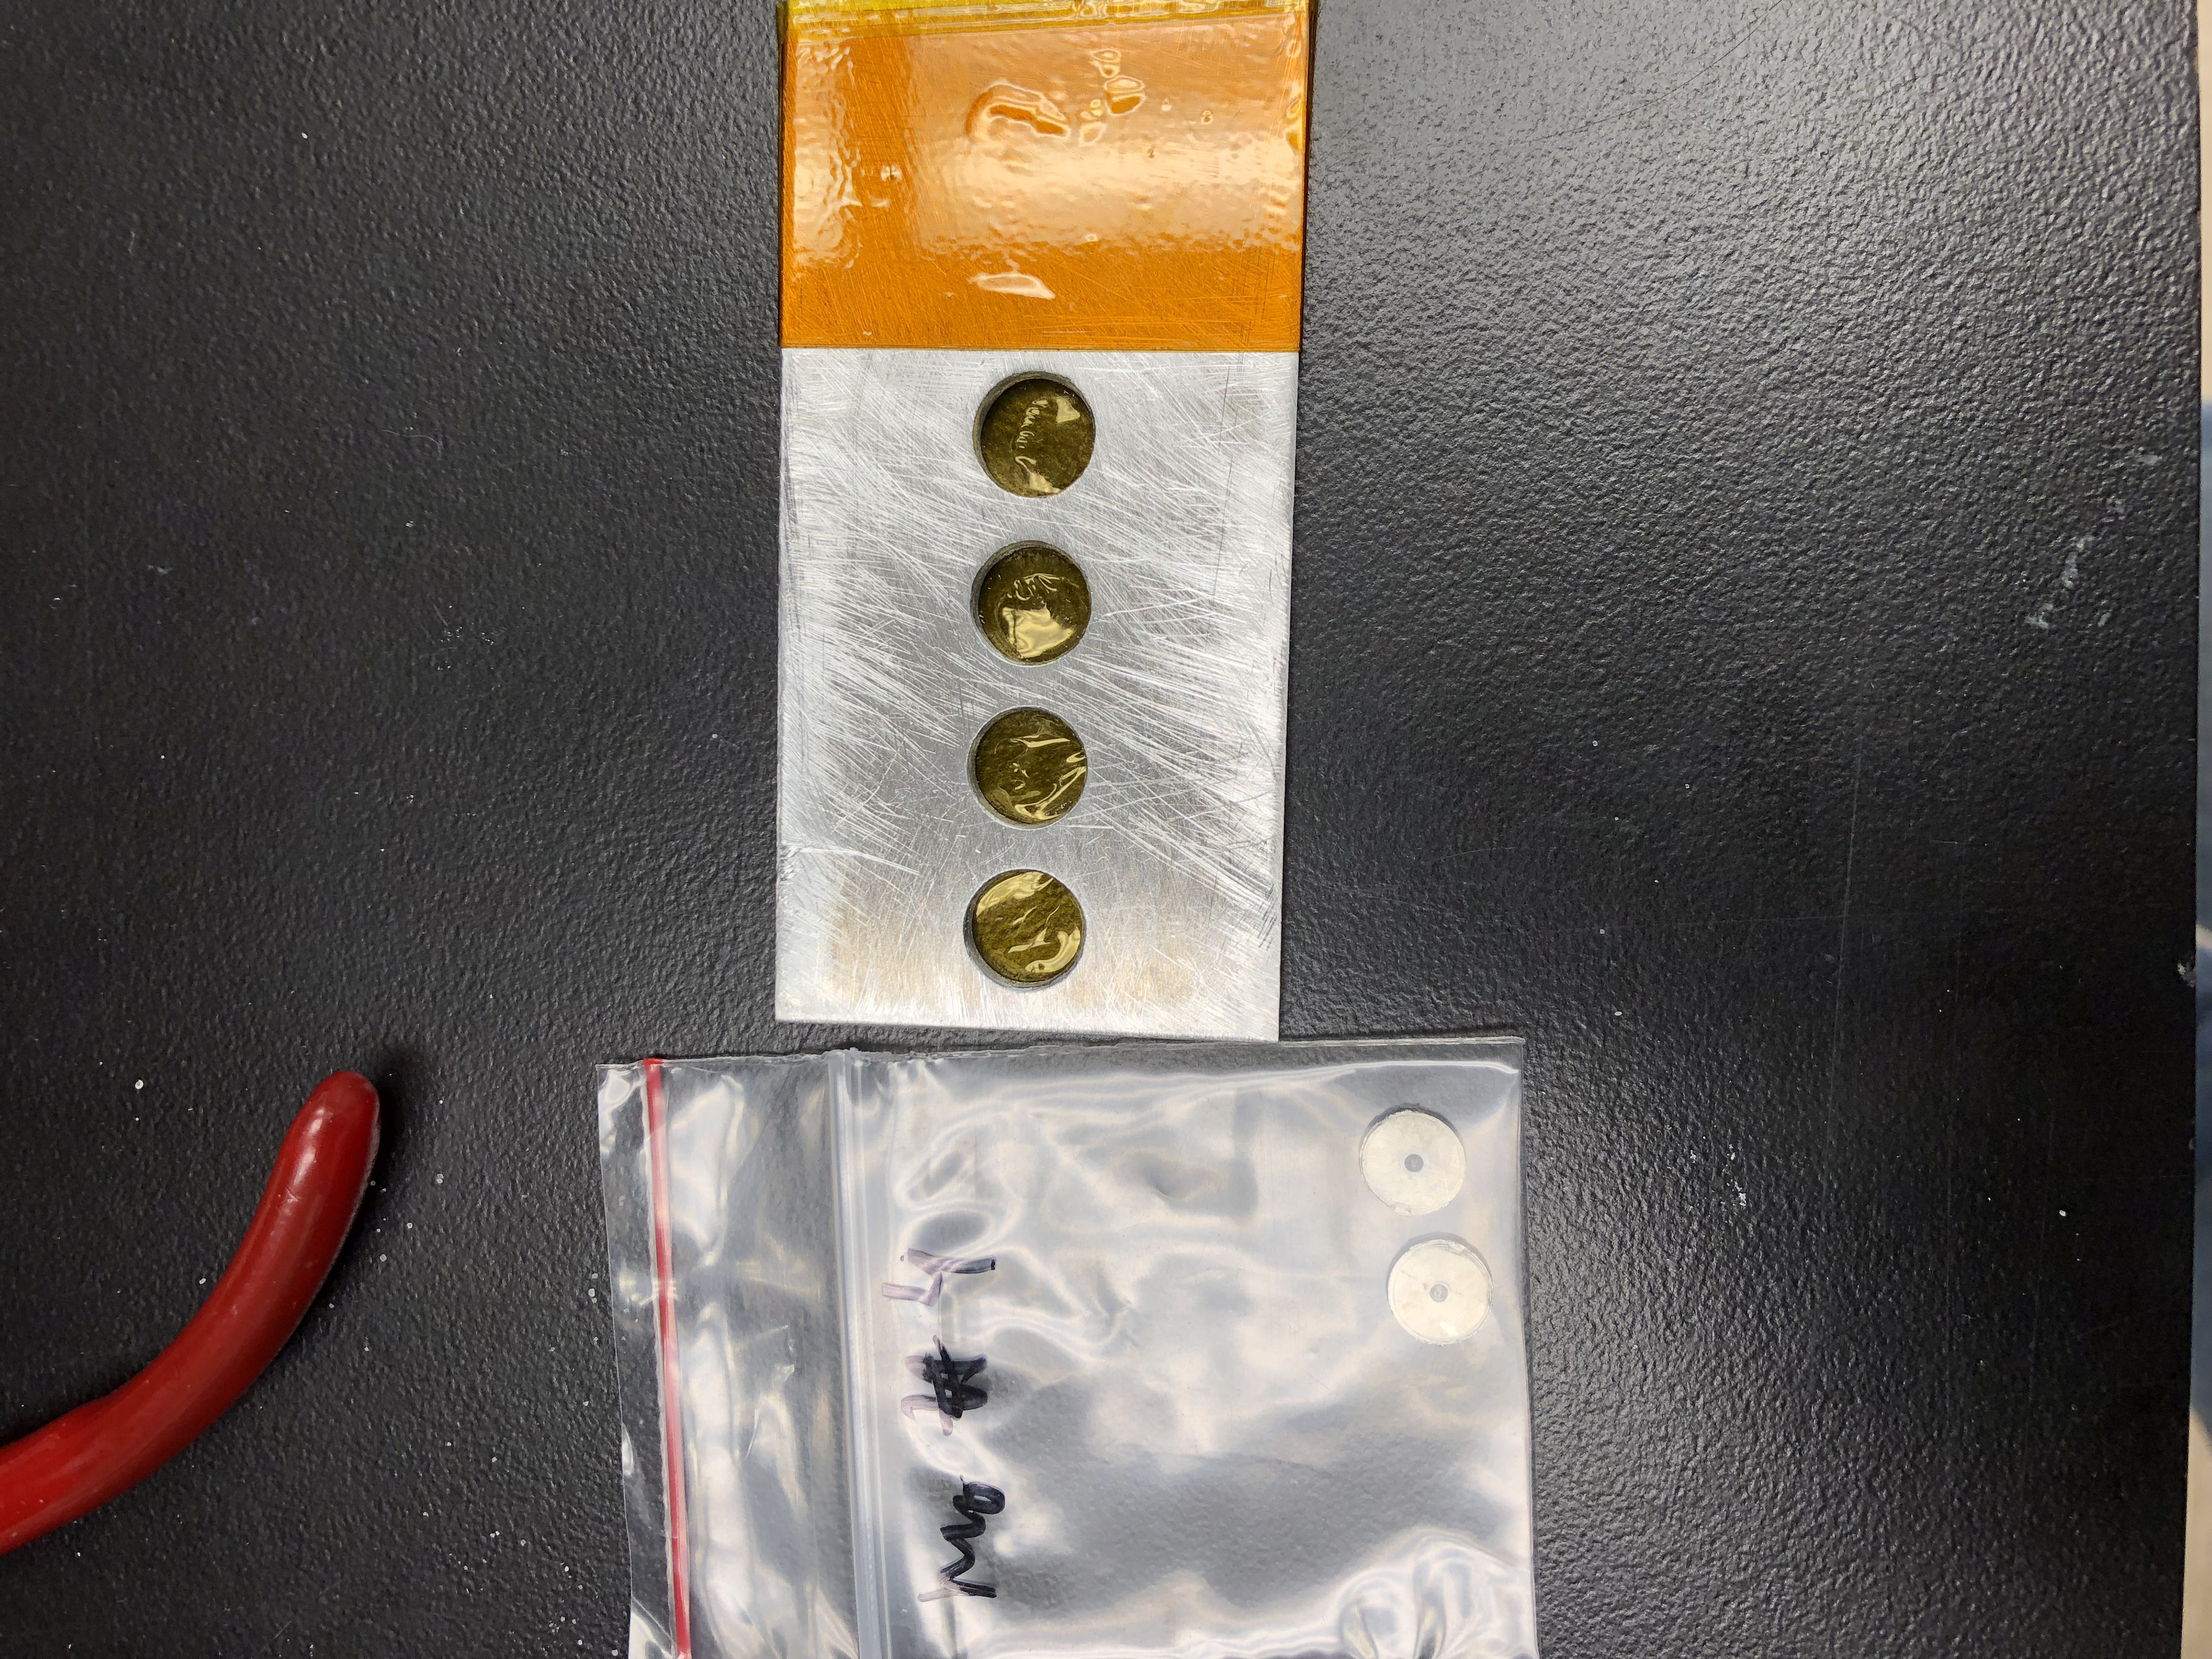
\includegraphics[width=0.75\columnwidth,angle=270]{./figures/IMG_8840.JPG}
 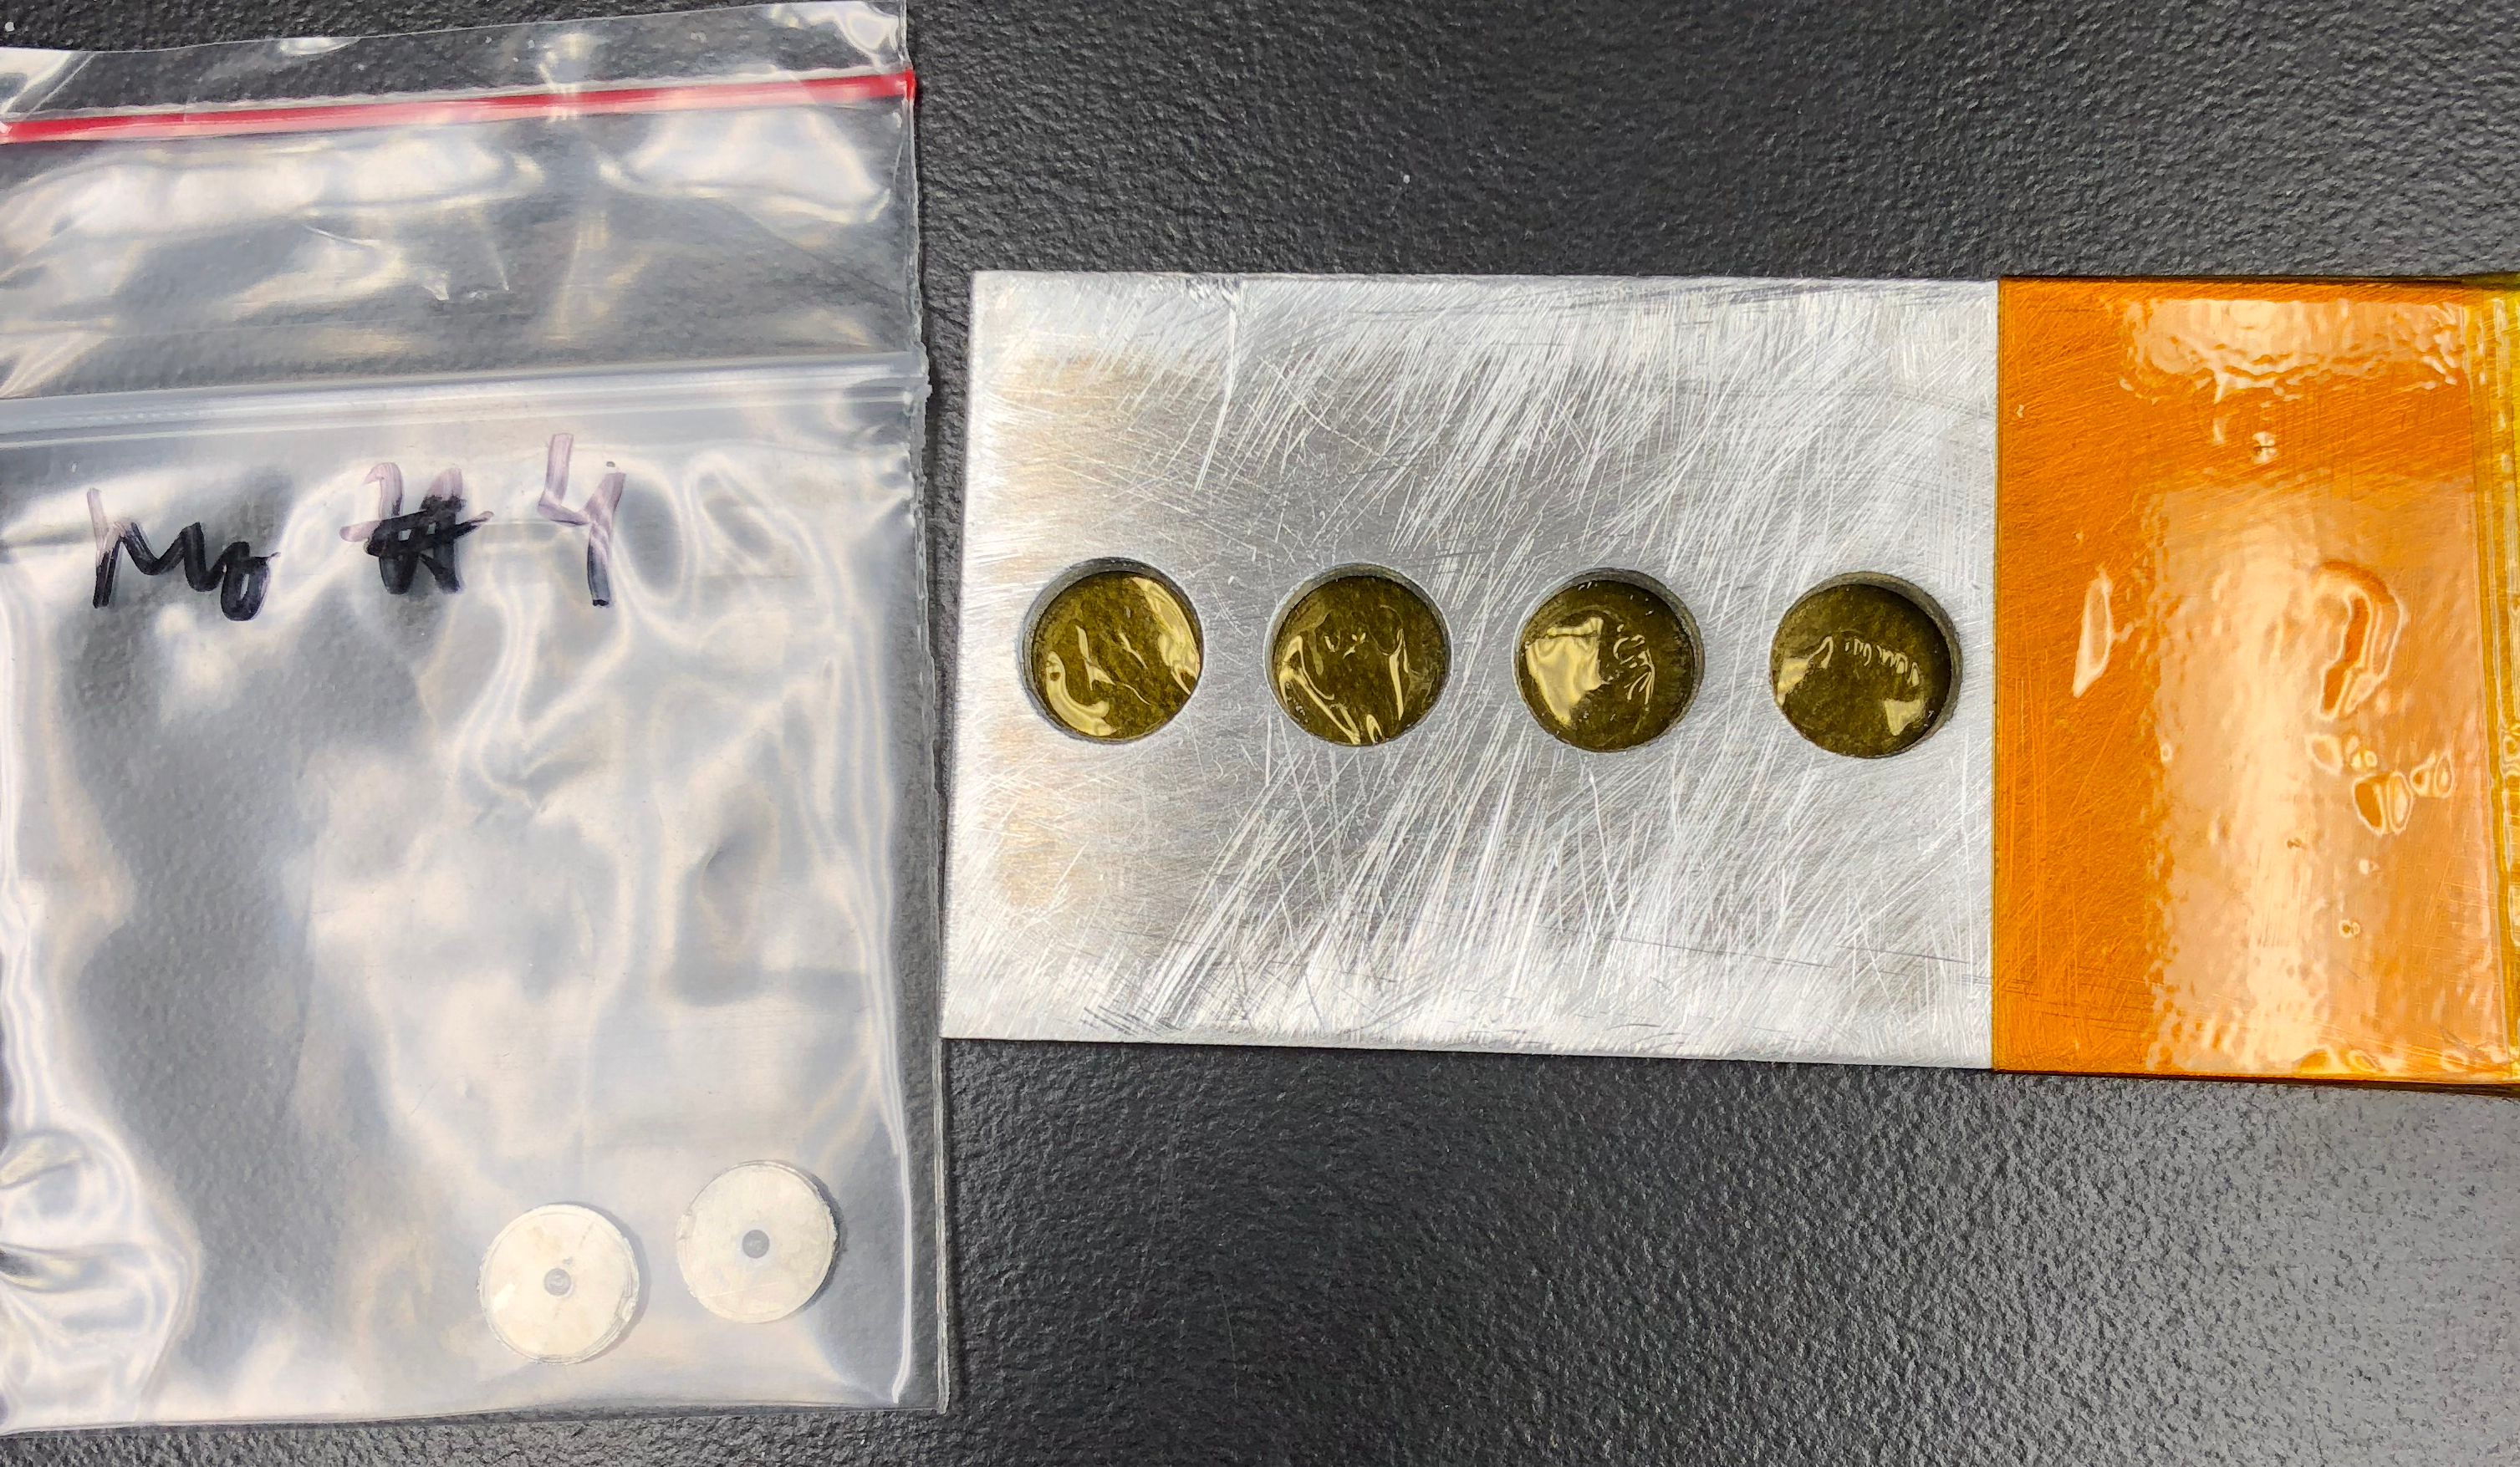
\includegraphics[width=0.75\columnwidth]{./figures/IMG_8840_cropped.JPG}
 % IMG_8840.JPG: 4032x3024 pixel, 72dpi, 142.24x106.68 cm, bb=0 0 4032 3024
 \caption{Custom target holder for the measurement of the \ce{^{98}Mo}(n,$\gamma$)\ce{^{99}Mo} cross section at four energy locations near 2.7\,MeV.}
 \label{fig:mo_4foils}
\end{figure}






With the capability established for precise (n,x) cross section measurements at the HFNG, a targeted experimental campaign is underway to address the needs of the nuclear data and applications communities.
Current and future experiments focus on the measurement of cross sections for a number of emerging  medical radionuclides, as well as novel production pathways for established radionuclides.
These include the \ce{^{32}S}(n,p)\ce{^{32}P}, \ce{^{67}Zn}(n,p)\ce{^{67}Cu}, \ce{^{89}Y}(n,p)\ce{^{89}Sr}, \ce{^{105}Pd}(n,p)\ce{^{105}Rh}, \ce{^{149}Sm}(n,p)\ce{^{149}Pm}, \ce{^{153}Eu}(n,p)\ce{^{153}Sm}, \ce{^{159}Tb}(n,p)\ce{^{159}Gd}, \ce{^{161}Dy}(n,p)\ce{^{161}Tb}, \\\ce{^{166}Er}(n,p)\ce{^{166}Ho}, \ce{^{169}Tm}(n,p)\ce{^{169}Er}, \ce{^{175}Lu}(n,p)\ce{^{175}Yb}, and \ce{^{177}Hf}(n,p)\ce{^{177}Lu} reactions.


